\documentclass[12 pt]{article}
\usepackage{amsmath}
\usepackage{amssymb}
\usepackage{geometry}
\usepackage{setspace}
\usepackage{graphicx}

\setlength{\emergencystretch}{15 pt}
\geometry{tmargin=2.5 cm, bmargin=2.5 cm, lmargin=2.5 cm, rmargin=2.5 cm}
\onehalfspacing

%\title{Spruce Budworm Work in Progress}
%\author{S\'ebastien Portalier}
%\date{January 2020}

\begin{document}
\begin{center}
\begin{Large}
\textbf{Diapause model for spruce budworms}\\
Portalier S\'ebastien, Candau Jean-No\"{e}l, and Lutscher Frithjof \\
\end{Large}
March 2nd, 2020
\end{center}
\begin{center}
\begin{large}
\textbf{Goal of the study}
\end{large}
\end{center}
The model focuses on the diapause stage. The aim of the study is to investigate the interplay between temperature and spruce budworm phenology. Especially, we focus on larvae survival (especially during "Winter" conditions) according to different temperature regimes and different scenario of stage transition (i.e. what determines the switch from a stage to another). Finally, we investigate how change in temperature may affect this system. 
\begin{center}
\begin{large}
\textbf{The model}
\end{large}
\end{center}
Let's consider the following development frame, with $t_0$ is time when eggs hatch, $t_d$ is time when diapause begins, $t_p$ is time when post-diapause begins, and $t_e$ is time at emergence (see figure 1). \par
\begin{figure}[h]
\begin{center}
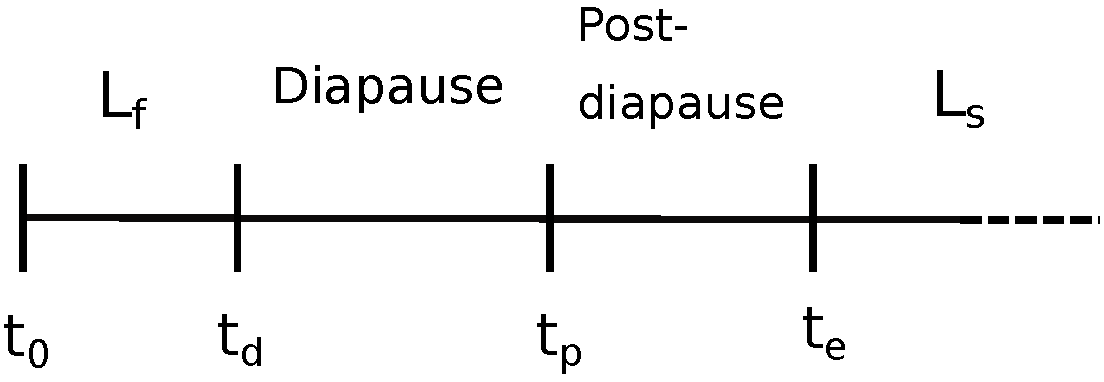
\includegraphics[width=12 cm, keepaspectratio]{Time_Line.pdf}
\caption{Time line of the model. $L_f$ is Fall stages, and $L_s$ are Summer stages.}
\end{center}
\end{figure}
\section{Fall stages}
Spruce budworm eggs hatch and $L_1$ and $L_2$ stages develop. Larvae don't feed but use energy for development. \par
The population starts with a given abundance ($L_f(t_0)$) and a given amount of energy ($E_f(t_0)$).
The system is:
\begin{equation}
    \left \lbrace
    \begin{array}{lcl}
        \Dot{E_f} & = & - \alpha _f T^{\beta _f} \\
        \dot{L_f} & = & - m_f (T) L_f
    \end{array} \right .
\end{equation}
where $T$ is temperature, $m_f$ is temperature-dependent mortality (to account for early freeze, for example), $\alpha _f$ and $\beta _f$ are constant that determine energy consumption according to temperature. 
Explicit solutions are:
\begin{equation}
    E_f (t) = E_f (t_0) - \int _{t_0} ^t \alpha _f T^{\beta _f} \; \mathrm{d}t \\
\end{equation}
and
\begin{equation}
    L_f (t) = \mathrm{e}^{- \int m_f(T(\sigma)) \; \mathrm{d}\sigma}L_f (t_0)
\end{equation}
The system runs until $t=t_d$. This event may be a fixed point in time (e.g. determined by photoperiod). But it may be dependent on larval development rate. In that case, development rate would be:
\begin{equation}\label{development}
\Dot{R_f}=r_f(T(t))
\end{equation}
where $R_f(t_0)=0$, and $R_f(t_d)=1$. 
\section{Diapause}
During diapause stage, larvae do not feed. They exhibit a low supercooling point. On the one hand, temperature has little to no effect on development rate, but on the other hand, energy consumption rate is still temperature-dependant. \par
The starting conditions are:
\begin{equation}
    \left \lbrace
    \begin{array}{lcl}
        E_d(t_d) & = & E_f(t_d) \\
        L_d(t_d) & = & L_f(t_d)
    \end{array} \right .
\end{equation}
and the system is:
\begin{equation}
    \left \lbrace
    \begin{array}{lcl}
        \Dot{E_d} & = & - \alpha _d T^{\beta _d} \\
        \dot{L_d} & = & - m_d (T) L_d
    \end{array} \right .
\end{equation}
Explicit solutions are:
\begin{equation}
    E_d (t) = E_d (t_d) - \int _{t_d} ^t \alpha _d T^{\beta _d} \; \mathrm{d}t \\
\end{equation}
and
\begin{equation}
    L_d (t) = \mathrm{e}^{- \int m_d(T(\sigma)) \; \mathrm{d}\sigma}L_d (t_p)
\end{equation}
However, mortality is low. From an extreme simplification point of view, we may assume that $m_d = 0$, if $T \geqslant \theta _d$, and that the whole population dies if $T < \theta _d$ during a certain period of time (e.g. more than 8 hours), where $\theta _d$ is the supercooling point of the diapause stage. In that case, $L_d (t_p) = L_d (t_d)$ if there is no freeze, and $0$ otherwise.\par
The system runs until $t=t_p$. This event may be triggered by:
\begin{itemize}
    \item \textbf{genetic}: the duration of the diapause stage is fixed. If the beginning of the diapause is determined by fixed external conditions (e.g. photoperiod), then the end of the diapause is also fixed. However, if the beginning of diapause varies (e.g. development rate of the Fall stages), then the end varies accordingly. 
    \item \textbf{photoperiod}: the end of diapause is a fixed moment in time (at a given location). Thus, if the begging of diapause is also induced by fixed external factors (e.g. photoperiod), its duration will be fixed, while if the beginning varies (e.g. development rate of Fall stage), its duration will also vary.
   \item \textbf{energy monitoring}: energy is used during diapause stage (and Fall stage). Rate of energy use is temperature-dependent. The end of diapause may be triggered when $E_d(t)<\phi _d$, where $\phi _d$ is the minimal amount of energy needed to continue into diapause.
    \item \textbf{temperature}: the end of diapause varies from year to year. The end of diapause may be triggered when $T> T_d$ during a certain period of time, where $T_d$ is the threshold temperature allowing the end of diapause. It may be determined by degree-days (i.e. the number of days where $T> T_d$).
\end{itemize}

\section{Post-diapause}
Larvae during post-diapause stage do not feed. They are more sensitive to temperature (e.g. they have a higher supercooling point),  and they have a different metabolic rate (energy use). \par
The starting conditions are:
\begin{equation}
    \left \lbrace
    \begin{array}{lcl}
        E_p(t_p) & = & E_d(t_p) \\
        L_p(t_p) & = & L_d(t_p)
    \end{array} \right .
\end{equation}
The system is:
\begin{equation}
    \left \lbrace
    \begin{array}{lcl}
        \Dot{E_p} & = & - \alpha _p T^{\beta _p} \\
        \dot{L_p} & = & - m_p(T) L_p
    \end{array} \right .
\end{equation}
Explicit solutions are:
\begin{equation}
    E_p (t) = E_p (t_p) - \int _{t_p} ^t \alpha _p T^{\beta _p} \; \mathrm{d}t \\
\end{equation}
and
\begin{equation}
    L_p (t) = \mathrm{e}^{- \int m_p(T(\sigma)) \; \mathrm{d}\sigma}L_p (t_p)
\end{equation}
Mortality varies with temperature (very high mortality if temperatures are low, since this stage is assumed to be less freeze-resistant). It may work in a similar way as diapause stage: the population dies if $T< \theta _p$ during a certain period of time, where $\theta _p$ is the supercooling temperature of the post-diapause stage. Otherwise, we may set up a $m_p(T)$ function that scales with the inverse of temperature (i.e. high mortality when temperature is low). \par
The system runs until $t=t_e$. This event is triggered by:
\begin{itemize}
    \item \textbf{temperature}: if $T> T_e$ during a certain period of time (e.g. number of days above temperature of emergence $T_e$).
    \item \textbf{energy}: if $E_p(t)< \phi _e$, where $\phi _e$ is the minimal amount of energy allowing to continue into post-diapause. The point is to determine if larvae would emerge if energy is below this threshold, or if they will die.
\end{itemize}
We may stop the model here or we can continue to the next stage. If we stop here, then food availability at $t=t_e$ will determine whether or not the population will survive.

\section{Summer stages}
The starting conditions are:
\begin{equation}
    \left \lbrace
       \begin{array}{lcl}
           E_s(t_e) & = & E_p(t_e) \\
           L_s(t_e) & = & L_p(t_e)
        \end{array} \right .    
\end{equation}
If food is available, we do not need to track energy anymore since larvae feed on the host. However, if food is not available yet, then energy has to be taken into account until food becomes available. \par
The model is:
\begin{equation}
    \left \lbrace
       \begin{array}{lcl}
           \Dot{E_s} & = & - \alpha _s T^{\beta _s} \\
           \dot{L_s} & = & - m_s(T,F) L_s
       \end{array} \right .
\end{equation}
where $F$ is food availability. If $E_s(t)<\phi _s$, where $\phi _s$ is the minimal amount of energy allowing the population to persist, then the population dies. If food becomes available only population abundance is taken into account.

\section{Questions}
\subsection{Beginning of diapause}
We assume that the beginning of the diapause stage ($t_d$) is a fixed point in time (early September). Is it a valid assumption? \par
Or should we assume that it may vary according to "hatching time" ($t_0$)? So, if eggs hatch (or are laid) later (earlier) in the year, diapause will occur later (earlier) as well. In that case, we probably need to include an equation for the developmental rate (equation 4). 
\subsection{Starting point of the model}
Do we need to consider the Fall stages? The only advantage of doing so would be to include special events such as early freeze (that would increase death) or unusually warm temperatures (that would increase energy consumption). \par
Otherwise, we may start directly at diapause ($t_d$). Hence, we may use different $L_d(t_d)$ and/or $E_d (t_d)$ to take Fall events into account as starting conditions instead of including them in the model explicitly. \par
If Fall stage is needed, then we should agree on $t_0$. Is it a fixed point in time?
\subsection{End point of the model}
Do we need to consider Summer stages? 
On the one hand, the model can relate the number of emerging larvae to the number of eggs laid (or larvae entering diapause, if we start at the diapause stage). If we want to know how many of these larvae will survive (until reproduction) in case of a mismatch between emergence and food availability, we need to consider Summer stages explicitly. \par
On the other hand, if we are only interested in the diapause stage and how much SBW can adapt to different climate/weather conditions, Summer stage may not be necessary. Hence, if we know when (within a year) food will be available at a given location, it should be enough knowing when larvae emerge from dormant stage to determine their ability to survive (i.e. how much time they will need to wait before food becomes available). Since we do not complete the full cycle, Summer stage may be ignored. \par
\subsection{Inter-individual variability}
Inter-individual variability may be included (which will increase the complexity of the model). It would play a role at each stage (i.e. how each individual react to the factor considered). For example, development rate (equation 4) can be written:
\begin{equation}\label{development}
\Dot{R_{fi}}=\delta _i r_f(T(t))
\end{equation}
where $r_f$ is average development rate, and $\delta _i$ is the individual $i$ variation on development rate relative to the average (i.e. if $\delta _i<1$, it develops slower than average, and if $\delta _i>1$, it develops faster than average). A similar approach may be used for the other stages.
\end{document}